\documentclass{extbook}[14pt]
\usepackage{multicol, enumerate, enumitem, hyperref, color, soul, setspace, parskip, fancyhdr, amssymb, amsthm, amsmath, bbm, latexsym, units, mathtools}
\everymath{\displaystyle}
\usepackage[headsep=0.5cm,headheight=0cm, left=1 in,right= 1 in,top= 1 in,bottom= 1 in]{geometry}
\usepackage{dashrule}  % Package to use the command below to create lines between items
\newcommand{\litem}[1]{\item #1

\rule{\textwidth}{0.4pt}}
\pagestyle{fancy}
\lhead{}
\chead{Answer Key for Progress Quiz 4 Version B}
\rhead{}
\lfoot{4378-7085}
\cfoot{}
\rfoot{Fall 2020}
\begin{document}
\textbf{This key should allow you to understand why you choose the option you did (beyond just getting a question right or wrong). \href{https://xronos.clas.ufl.edu/mac1105spring2020/courseDescriptionAndMisc/Exams/LearningFromResults}{More instructions on how to use this key can be found here}.}

\textbf{If you have a suggestion to make the keys better, \href{https://forms.gle/CZkbZmPbC9XALEE88}{please fill out the short survey here}.}

\textit{Note: This key is auto-generated and may contain issues and/or errors. The keys are reviewed after each exam to ensure grading is done accurately. If there are issues (like duplicate options), they are noted in the offline gradebook. The keys are a work-in-progress to give students as many resources to improve as possible.}

\rule{\textwidth}{0.4pt}

\begin{enumerate}\litem{
Describe the end behavior of the polynomial below.
\[ f(x) = -7(x + 8)^{3}(x - 8)^{6}(x + 2)^{3}(x - 2)^{3} \]
The solution is the graph below, which is option A.
\begin{center}
    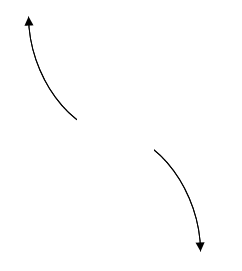
\includegraphics[width=0.3\textwidth]{../Figures/polyEndBehaviorCopyAB.png}
\end{center}\begin{enumerate}[label=\Alph*.]
\begin{multicols}{2}
\item 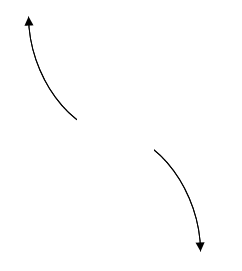
\includegraphics[width = 0.3\textwidth]{../Figures/polyEndBehaviorCopyAB.png}
\item 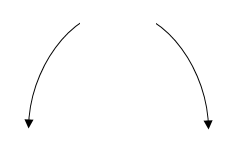
\includegraphics[width = 0.3\textwidth]{../Figures/polyEndBehaviorCopyBB.png}
\item 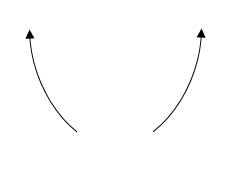
\includegraphics[width = 0.3\textwidth]{../Figures/polyEndBehaviorCopyCB.png}
\item 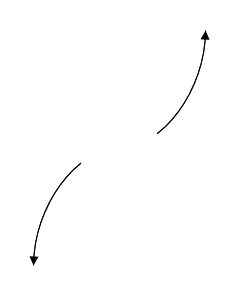
\includegraphics[width = 0.3\textwidth]{../Figures/polyEndBehaviorCopyDB.png}
\end{multicols}\item None of the above.\end{enumerate}
\textbf{General Comment:} Remember that end behavior is determined by the leading coefficient AND whether the \textbf{sum} of the multiplicities is positive or negative.
}
\litem{
Construct the lowest-degree polynomial given the zeros below. Then, choose the intervals that contain the coefficients of the polynomial in the form $ax^3+bx^2+cx+d$.
\[ \frac{-4}{5}, \frac{-1}{5}, \text{ and } \frac{-4}{3} \]
The solution is \( 75x^{3} +175 x^{2} +112 x + 16 \), which is option B.\begin{enumerate}[label=\Alph*.]
\item \( a \in [74, 76], b \in [53, 57], c \in [-76, -63], \text{ and } d \in [-16, -13] \)

$75x^{3} +55 x^{2} -72 x -16$, which corresponds to multiplying out $(5x + 5)(5x -5)(3x -3)$.
\item \( a \in [74, 76], b \in [175, 179], c \in [112, 115], \text{ and } d \in [16, 17] \)

* $75x^{3} +175 x^{2} +112 x + 16$, which is the correct option.
\item \( a \in [74, 76], b \in [175, 179], c \in [112, 115], \text{ and } d \in [-16, -13] \)

$75x^{3} +175 x^{2} +112 x -16$, which corresponds to multiplying everything correctly except the constant term.
\item \( a \in [74, 76], b \in [-175, -173], c \in [112, 115], \text{ and } d \in [-16, -13] \)

$75x^{3} -175 x^{2} +112 x -16$, which corresponds to multiplying out $(5x -4)(5x -1)(3x -4)$.
\item \( a \in [74, 76], b \in [22, 27], c \in [-91, -82], \text{ and } d \in [16, 17] \)

$75x^{3} +25 x^{2} -88 x + 16$, which corresponds to multiplying out $(5x + 5)(5x + 5)(3x -3)$.
\end{enumerate}

\textbf{General Comment:} To construct the lowest-degree polynomial, you want to multiply out $(5x + 4)(5x + 1)(3x + 4)$
}
\litem{
Describe the zero behavior of the zero $x = 5$ of the polynomial below.
\[ f(x) = 2(x + 5)^{9}(x - 5)^{14}(x + 4)^{3}(x - 4)^{4} \]
The solution is the graph below, which is option C.
\begin{center}
    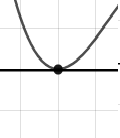
\includegraphics[width=0.3\textwidth]{../Figures/polyZeroBehaviorCB.png}
\end{center}\begin{enumerate}[label=\Alph*.]
\begin{multicols}{2}
\item 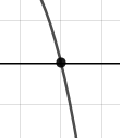
\includegraphics[width = 0.3\textwidth]{../Figures/polyZeroBehaviorAB.png}
\item 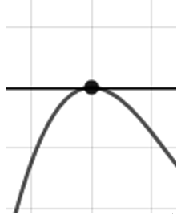
\includegraphics[width = 0.3\textwidth]{../Figures/polyZeroBehaviorBB.png}
\item 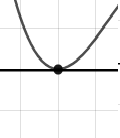
\includegraphics[width = 0.3\textwidth]{../Figures/polyZeroBehaviorCB.png}
\item 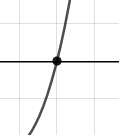
\includegraphics[width = 0.3\textwidth]{../Figures/polyZeroBehaviorDB.png}
\end{multicols}\item None of the above.\end{enumerate}
\textbf{General Comment:} You will need to sketch the entire graph, then zoom in on the zero the question asks about.
}
\litem{
Describe the end behavior of the polynomial below.
\[ f(x) = 7(x + 8)^{5}(x - 8)^{8}(x - 5)^{4}(x + 5)^{4} \]
The solution is the graph below, which is option D.
\begin{center}
    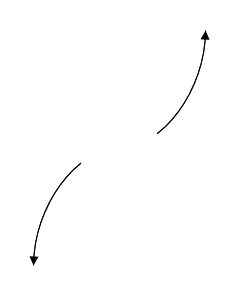
\includegraphics[width=0.3\textwidth]{../Figures/polyEndBehaviorDB.png}
\end{center}\begin{enumerate}[label=\Alph*.]
\begin{multicols}{2}
\item 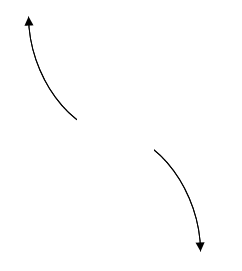
\includegraphics[width = 0.3\textwidth]{../Figures/polyEndBehaviorAB.png}
\item 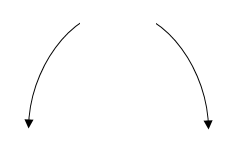
\includegraphics[width = 0.3\textwidth]{../Figures/polyEndBehaviorBB.png}
\item 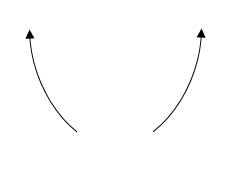
\includegraphics[width = 0.3\textwidth]{../Figures/polyEndBehaviorCB.png}
\item 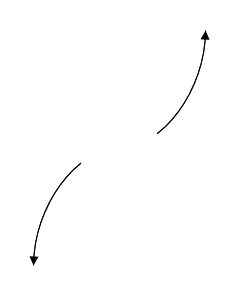
\includegraphics[width = 0.3\textwidth]{../Figures/polyEndBehaviorDB.png}
\end{multicols}\item None of the above.\end{enumerate}
\textbf{General Comment:} Remember that end behavior is determined by the leading coefficient AND whether the \textbf{sum} of the multiplicities is positive or negative.
}
\litem{
Construct the lowest-degree polynomial given the zeros below. Then, choose the intervals that contain the coefficients of the polynomial in the form $x^3+bx^2+cx+d$.
\[ 3 + 4 i \text{ and } -3 \]
The solution is \( x^{3} -3 x^{2} +7 x + 75 \), which is option A.\begin{enumerate}[label=\Alph*.]
\item \( b \in [-6.9, -0.4], c \in [5.58, 7.49], \text{ and } d \in [71.2, 77.6] \)

* $x^{3} -3 x^{2} +7 x + 75$, which is the correct option.
\item \( b \in [-0.2, 1.3], c \in [-0.66, 2.32], \text{ and } d \in [-10.7, -7.6] \)

$x^{3} + x^{2} -9$, which corresponds to multiplying out $(x -3)(x + 3)$.
\item \( b \in [1.9, 4.8], c \in [5.58, 7.49], \text{ and } d \in [-77.3, -73.5] \)

$x^{3} +3 x^{2} +7 x -75$, which corresponds to multiplying out $(x-(3 + 4 i))(x-(3 - 4 i))(x -3)$.
\item \( b \in [-0.2, 1.3], c \in [-2.47, -0.78], \text{ and } d \in [-13.7, -9.8] \)

$x^{3} + x^{2} -x -12$, which corresponds to multiplying out $(x -4)(x + 3)$.
\item \( \text{None of the above.} \)

This corresponds to making an unanticipated error or not understanding how to use nonreal complex numbers to create the lowest-degree polynomial. If you chose this and are not sure what you did wrong, please contact the coordinator for help.
\end{enumerate}

\textbf{General Comment:} Remember that the conjugate of $a+bi$ is $a-bi$. Since these zeros always come in pairs, we need to multiply out $(x-(3 + 4 i))(x-(3 - 4 i))(x-(-3))$.
}
\litem{
Construct the lowest-degree polynomial given the zeros below. Then, choose the intervals that contain the coefficients of the polynomial in the form $ax^3+bx^2+cx+d$.
\[ -7, \frac{1}{3}, \text{ and } \frac{5}{2} \]
The solution is \( 6x^{3} +25 x^{2} -114 x + 35 \), which is option D.\begin{enumerate}[label=\Alph*.]
\item \( a \in [4, 11], b \in [-55, -52], c \in [80, 87], \text{ and } d \in [29, 36] \)

$6x^{3} -55 x^{2} +86 x + 35$, which corresponds to multiplying out $(x + 1)(3x + 3)(2x -2)$.
\item \( a \in [4, 11], b \in [-66, -57], c \in [118, 125], \text{ and } d \in [-41, -31] \)

$6x^{3} -59 x^{2} +124 x -35$, which corresponds to multiplying out $(x + 1)(3x -3)(2x -2)$.
\item \( a \in [4, 11], b \in [-25, -20], c \in [-122, -107], \text{ and } d \in [-41, -31] \)

$6x^{3} -25 x^{2} -114 x -35$, which corresponds to multiplying out $(x -7)(3x + 1)(2x + 5)$.
\item \( a \in [4, 11], b \in [19, 27], c \in [-122, -107], \text{ and } d \in [29, 36] \)

* $6x^{3} +25 x^{2} -114 x + 35$, which is the correct option.
\item \( a \in [4, 11], b \in [19, 27], c \in [-122, -107], \text{ and } d \in [-41, -31] \)

$6x^{3} +25 x^{2} -114 x -35$, which corresponds to multiplying everything correctly except the constant term.
\end{enumerate}

\textbf{General Comment:} To construct the lowest-degree polynomial, you want to multiply out $(x + 7)(3x -1)(2x -5)$
}
\litem{
Which of the following equations \textit{could} be of the graph presented below?

\begin{center}
    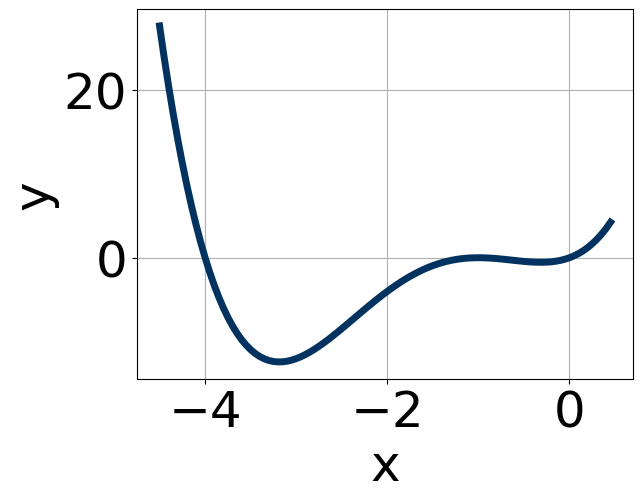
\includegraphics[width=0.5\textwidth]{../Figures/polyGraphToFunctionCopyB.png}
\end{center}



The solution is \( -20x^{7} (x + 1)^{5} (x + 2)^{9} \), which is option D.\begin{enumerate}[label=\Alph*.]
\item \( 7x^{9} (x + 1)^{7} (x + 2)^{5} \)

This corresponds to the leading coefficient being the opposite value than it should be.
\item \( -7x^{9} (x + 1)^{10} (x + 2)^{11} \)

The factor $-1$ should have been an odd power.
\item \( 3x^{11} (x + 1)^{8} (x + 2)^{7} \)

The factor $(x + 1)$ should have an odd power and the leading coefficient should be the opposite sign.
\item \( -20x^{7} (x + 1)^{5} (x + 2)^{9} \)

* This is the correct option.
\item \( -3x^{5} (x + 1)^{10} (x + 2)^{8} \)

The factors $-1$ and $-2$ have have been odd power.
\end{enumerate}

\textbf{General Comment:} General Comments: Draw the x-axis to determine which zeros are touching (and so have even multiplicity) or cross (and have odd multiplicity).
}
\litem{
Describe the zero behavior of the zero $x = 3$ of the polynomial below.
\[ f(x) = 8(x - 6)^{11}(x + 6)^{8}(x + 3)^{7}(x - 3)^{2} \]
The solution is the graph below, which is option B.
\begin{center}
    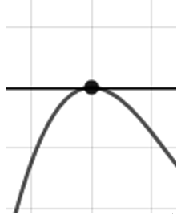
\includegraphics[width=0.3\textwidth]{../Figures/polyZeroBehaviorCopyBB.png}
\end{center}\begin{enumerate}[label=\Alph*.]
\begin{multicols}{2}
\item 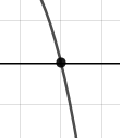
\includegraphics[width = 0.3\textwidth]{../Figures/polyZeroBehaviorCopyAB.png}
\item 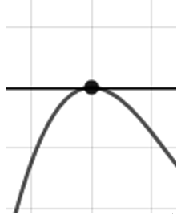
\includegraphics[width = 0.3\textwidth]{../Figures/polyZeroBehaviorCopyBB.png}
\item 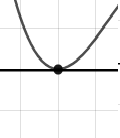
\includegraphics[width = 0.3\textwidth]{../Figures/polyZeroBehaviorCopyCB.png}
\item 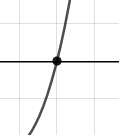
\includegraphics[width = 0.3\textwidth]{../Figures/polyZeroBehaviorCopyDB.png}
\end{multicols}\item None of the above.\end{enumerate}
\textbf{General Comment:} You will need to sketch the entire graph, then zoom in on the zero the question asks about.
}
\litem{
Construct the lowest-degree polynomial given the zeros below. Then, choose the intervals that contain the coefficients of the polynomial in the form $x^3+bx^2+cx+d$.
\[ -4 + 4 i \text{ and } 4 \]
The solution is \( x^{3} +4 x^{2} -128 \), which is option D.\begin{enumerate}[label=\Alph*.]
\item \( b \in [-2.3, 2.2], c \in [-3, 10], \text{ and } d \in [-22, -15] \)

$x^{3} + x^{2} -16$, which corresponds to multiplying out $(x + 4)(x -4)$.
\item \( b \in [-2.3, 2.2], c \in [-14, -6], \text{ and } d \in [11, 19] \)

$x^{3} + x^{2} -8 x + 16$, which corresponds to multiplying out $(x -4)(x -4)$.
\item \( b \in [-5.4, -1], c \in [-3, 10], \text{ and } d \in [123, 134] \)

$x^{3} -4 x^{2} + 128$, which corresponds to multiplying out $(x-(-4 + 4 i))(x-(-4 - 4 i))(x + 4)$.
\item \( b \in [2.1, 5.3], c \in [-3, 10], \text{ and } d \in [-138, -126] \)

* $x^{3} +4 x^{2} -128$, which is the correct option.
\item \( \text{None of the above.} \)

This corresponds to making an unanticipated error or not understanding how to use nonreal complex numbers to create the lowest-degree polynomial. If you chose this and are not sure what you did wrong, please contact the coordinator for help.
\end{enumerate}

\textbf{General Comment:} Remember that the conjugate of $a+bi$ is $a-bi$. Since these zeros always come in pairs, we need to multiply out $(x-(-4 + 4 i))(x-(-4 - 4 i))(x-(4))$.
}
\litem{
Which of the following equations \textit{could} be of the graph presented below?

\begin{center}
    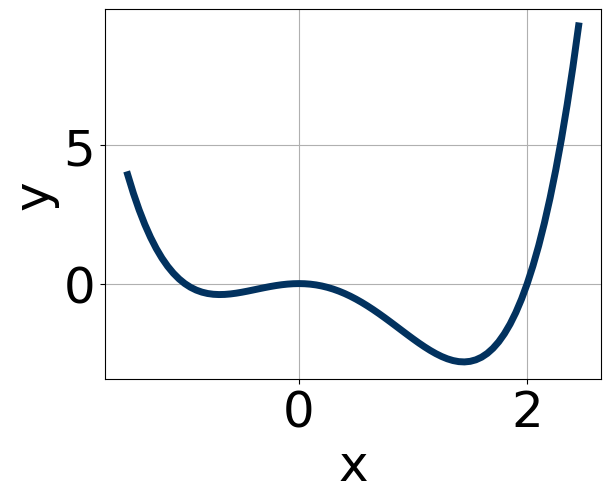
\includegraphics[width=0.5\textwidth]{../Figures/polyGraphToFunctionB.png}
\end{center}



The solution is \( 3x^{5} (x + 3)^{9} (x - 2)^{5} \), which is option E.\begin{enumerate}[label=\Alph*.]
\item \( 9x^{8} (x + 3)^{6} (x - 2)^{11} \)

The factors $-3$ and $0$ have have been odd power.
\item \( 10x^{9} (x + 3)^{6} (x - 2)^{11} \)

The factor $-3$ should have been an odd power.
\item \( -14x^{11} (x + 3)^{10} (x - 2)^{7} \)

The factor $(x + 3)$ should have an odd power and the leading coefficient should be the opposite sign.
\item \( -10x^{9} (x + 3)^{5} (x - 2)^{7} \)

This corresponds to the leading coefficient being the opposite value than it should be.
\item \( 3x^{5} (x + 3)^{9} (x - 2)^{5} \)

* This is the correct option.
\end{enumerate}

\textbf{General Comment:} General Comments: Draw the x-axis to determine which zeros are touching (and so have even multiplicity) or cross (and have odd multiplicity).
}
\end{enumerate}

\end{document}